\documentclass[mathserif]{beamer}
% \includeonlyframes{current}                                    
\input{macro}                       
\usetheme{camp}

%packages
\usepackage{graphicx}
\usepackage{tikz}
\usepackage{pgfplots}
\tikzset{>=stealth}
\usepackage{hyperref}
\usepackage{xcolor}

\usepackage{setspace}

\usepackage[ampersand]{easylist}

\usepackage{amsmath}
\usepackage{mathtools}

%informations about talk
\title[Energy Minimization via Graph Cuts ]{Fast Approximate Energy Minimization \\via Graph Cuts}
\author[Felix Wechsler]{Felix Wechsler}
\institute[CAMP]{Computer Aided Medical Procedures \\Technische Universit\"at M\"unchen}
\date[]{\today}

\usepackage[autocite=footnote,backend=biber, citestyle=authortitle, maxnames=99,maxalphanames=5]{biblatex}
\addbibresource{../common/references.bib}

\def\pl{\mathcal{P}}

\def\secslide{
    \begin{frame}
        \centering \Huge \secname
    \end{frame}
    \addtocounter{framenumber}{-1}
}


%fuer appendix right slide number
\newcommand{\appendixStart}{
        \newcounter{frameNumbersMain}
            \setcounter{frameNumbersMain}{\value{framenumber}}
                \begin{frame}
                        \centering
                        \Huge Appendix
                \end{frame}
    \addtocounter{framenumber}{-1}
}
\newcommand{\appendixEnd}{
        \setcounter{framenumber}{\value{frameNumbersMain}}
}


%start of document
\begin{document}


\begin{frame}
    \titlepage
\end{frame}


\begin{frame}{Outline}
    \tableofcontents
    \small
    Used paper: \cite{paper}
\end{frame}

    
\section{Basics}
\secslide
\begin{frame}{Standard CV Problem}
    \begin{itemize}
        \item Tackling noisy images
        \item Piecewise smooth variation of intensity 
    \end{itemize}
    $\implies$ energy minimization 
    \vspace{1cm}
    \begin{columns}
        \begin{column}{.4\textwidth}
            \centering
            \includegraphics[width=.7\textwidth]{../testimages/Lena/Lenna_500_40percent.png}
        \end{column}
        \begin{column}{0.2\textwidth}
            \centering
            \visible<2>{
            \scalebox{0.7}{
                
\begin{tikzpicture}
                    \fill[color=black] (1,0) --(3,0) --(3,1) --(4.5,-1) -- (3,-3) -- (3, -2) -- (1,-2);
                \end{tikzpicture}}
            }
        \end{column}
        \begin{column}{.4\textwidth}
            \centering
            \visible<2>{
                \includegraphics[width=.7\textwidth]{../testimages/Lena/Lenna_500.png}
            }
        \end{column}
    \end{columns}
\end{frame}

\begin{frame}{Labeling}
    \begin{itemize}
        \item Every pixel $p \in \mathcal{P}$ has label $f_p \in \mathcal{L}$
        \item Labeling of image is called $f$
        \item Label is intensity in image restoration
    \end{itemize}
    \vspace{1cm}
    \begin{columns}
        \begin{column}{0.45\textwidth}
            \centering
            \begin{tikzpicture}
                \def\sqwi{0.6}
                \def\sechs{black!100!white}
                \def\funf{black!90!white}
                \def\vier{black!60!white}
                \def\zwei{black!35!white}
                \def\eins{black!10!white}
                \def\null{black!0!white}
                        \draw (-0.65,-0.05) rectangle (1.55,2.15);
                    \only<1,4>{
                        \draw[color=\funf, fill] (0,0) rectangle node{5} (0-\sqwi,0+\sqwi);
                        \draw[color=\vier, fill] (0.75,0) rectangle node{4} (0.75-\sqwi,0+\sqwi);
                        \draw[color=\funf, fill] (1.5,0) rectangle node{5} (1.5-\sqwi,0+\sqwi);
                        \draw[color=\zwei, fill] (0,0.75) rectangle node{2} (0-\sqwi,0.75+\sqwi);
                        \draw[color=\eins, fill] (0.75,0.75) rectangle node{1} (0.75-\sqwi,0.75+\sqwi);
                        \draw[color=\funf, fill] (1.5,0.75) rectangle node{5} (1.5-\sqwi,0.75+\sqwi);
                        \draw[color=\sechs,fill] (0,1.5) rectangle node{6} (0-\sqwi,1.5+\sqwi);
                        \draw[color=\vier, fill] (0.75,1.5) rectangle node{4} (0.75-\sqwi,1.5+\sqwi);
                        \draw[color=\funf, fill] (1.5,1.5) rectangle node{5} (1.5-\sqwi,1.5+\sqwi);
                    }%                    
                        \only<2-3>{
                        \draw (-0.65,-0.05) rectangle (1.55,2.15);
                        \draw[color=black] (0,0) rectangle node{5} (0-\sqwi,0+\sqwi);
                        \draw[color=black] (0.75,0) rectangle node{4} (0.75-\sqwi,0+\sqwi);
                        \draw[color=black] (1.5,0) rectangle node{5} (1.5-\sqwi,0+\sqwi);
                        \draw[color=black] (0,0.75) rectangle node{2} (0-\sqwi,0.75+\sqwi);
                        \draw[color=black] (0.75,0.75) rectangle node{1} (0.75-\sqwi,0.75+\sqwi);
                        \draw[color=black] (1.5,0.75) rectangle node{5} (1.5-\sqwi,0.75+\sqwi);
                        \draw[color=black] (0,1.5) rectangle node{6} (0-\sqwi,1.5+\sqwi);
                        \draw[color=black] (0.75,1.5) rectangle node{4} (0.75-\sqwi,1.5+\sqwi);
                        \draw[color=black] (1.5,1.5) rectangle node{5} (1.5-\sqwi,1.5+\sqwi);
                    }
            \end{tikzpicture}
            \\
            labeling $f$
        \end{column}
        \begin{column}{0.2\textwidth}
            \centering
            \scalebox{0.7}{
            
\begin{tikzpicture}
                \only<3->{
                \fill[color=black] (1,0) --(3,0) --(3,1) --(4.5,-1) -- (3,-3) -- (3, -2) -- (1,-2);
                }
            \end{tikzpicture}}
        \end{column}
        \begin{column}{0.45\textwidth}
            \centering
            
\begin{tikzpicture}
                \def\sqwi{0.6}
                \def\sqwi{0.6}
                \def\sechs{black!100!white}
                \def\funf{black!90!white}
                \def\vier{black!60!white}
                \def\zwei{black!35!white}
                \def\eins{black!10!white}
                \def\null{black!0!white}
                \only<3>{ 
                        \draw (-0.65,-0.05) rectangle (1.55,2.15);
                        \draw[color=black] (0,0) rectangle node{5} (0-\sqwi,0+\sqwi);
                        \draw[color=black] (0.75,0) rectangle node{4} (0.75-\sqwi,0+\sqwi);
                        \draw[color=black] (1.5,0) rectangle node{5} (1.5-\sqwi,0+\sqwi);
                        \draw[color=black] (0,0.75) rectangle node{4} (0-\sqwi,0.75+\sqwi);
                        \draw[color=black] (0.75,0.75) rectangle node{4} (0.75-\sqwi,0.75+\sqwi);
                        \draw[color=black] (1.5,0.75) rectangle node{5} (1.5-\sqwi,0.75+\sqwi);
                        \draw[color=black] (0,1.5) rectangle node{5} (0-\sqwi,1.5+\sqwi);
                        \draw[color=black] (0.75,1.5) rectangle node{4} (0.75-\sqwi,1.5+\sqwi);
                        \draw[color=black] (1.5,1.5) rectangle node{5} (1.5-\sqwi,1.5+\sqwi);
                }%
                \only<4>{
                        \draw (-0.65,-0.05) rectangle (1.55,2.15);
                        \draw[color=\funf, fill] (0,0) rectangle node{5} (0-\sqwi,0+\sqwi);
                        \draw[color=\vier, fill] (0.75,0) rectangle node{4} (0.75-\sqwi,0+\sqwi);
                        \draw[color=\funf, fill] (1.5,0) rectangle node{5} (1.5-\sqwi,0+\sqwi);
                        \draw[color=\vier, fill] (0,0.75) rectangle node{4} (0-\sqwi,0.75+\sqwi);
                        \draw[color=\vier, fill] (0.75,0.75) rectangle node{4} (0.75-\sqwi,0.75+\sqwi);
                        \draw[color=\funf, fill] (1.5,0.75) rectangle node{5} (1.5-\sqwi,0.75+\sqwi);
                        \draw[color=\funf, fill] (0,1.5) rectangle node{5} (0-\sqwi,1.5+\sqwi);
                        \draw[color=\vier, fill] (0.75,1.5) rectangle node{4} (0.75-\sqwi,1.5+\sqwi);
                        \draw[color=\funf, fill] (1.5,1.5) rectangle node{5} (1.5-\sqwi,1.5+\sqwi);
                }
            \end{tikzpicture}
            \\
            \only<3-4>{
            labeling $\hat f$}
        \end{column}
    \end{columns}
\end{frame}


\begin{frame}{Energy Function}
    \begin{equation}
        E(f) = E_\text{smooth}(f) + E_\text{data}(f)
    \end{equation}
    \begin{itemize}
        \item $E_\text{smooth}$ $\hat=$ smoothness of image
        \item $E_\text{data}$ $\hat=$ disagreement between $f$ and image data
    \end{itemize}
    \begin{equation}
        E_\text{data} = \sum_{p \in \pl}^{} D_p(f_p)
    \end{equation}
    \begin{itemize}
        \item i.e.: $D_p(f_p) = (f_p-i_p)^2$ 
    \end{itemize}
    \footnotesize
    \begin{itemize}
        \item[] $f_p$ label pixel $p$
        \item[] $i_p$ original intensity of pixel p
    \end{itemize}
\end{frame}

\begin{frame}[label=current]{Smoothness Term}
    \begin{equation}
        E_\text{smooth} = \sum_{ \{p,q\} \in \mathcal{N}} V_{p,q}(f_p,f_q)
    \end{equation}
        
    \begin{columns}
        
        \begin{column}{.8\textwidth} 
            \begin{itemize}
                \item $V_{p,q}$: potential function
                \item $\mathcal{N}$: set of pair of adjacent pixels
                % \item semi-metric: $V(\alpha, \beta) = V(\beta, \alpha) \geq 0$ and $V(\alpha,\beta) = 0 \Leftrightarrow \alpha=\beta$ 
                % \item metric: $V(\alpha, \beta) \leq V(\alpha,\gamma)+V(\gamma,\beta)$ 
                % \item $\alpha$-$\beta$-swap move algorithm for semi-metric
                % \item $\alpha$-expansion move algorithm for metric
                % \item for $E_\text{smooth}$ many functions are possible
            \end{itemize}

         
        \end{column}
        \begin{column}{0.2\textwidth}
            \centering
            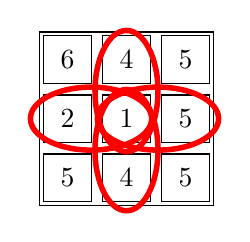
\begin{tikzpicture}
                \def\sqwi{0.6}
                        \draw (-0.65,-0.05) rectangle (1.55,2.15);
                        \draw[color=black] (0,0) rectangle node{5} (0-\sqwi,0+\sqwi);
                        \draw[color=black] (0.75,0) rectangle node{4} (0.75-\sqwi,0+\sqwi);
                        \draw[color=black] (1.5,0) rectangle node{5} (1.5-\sqwi,0+\sqwi);
                        \draw[color=black] (0,0.75) rectangle node{2} (0-\sqwi,0.75+\sqwi);
                        \draw[color=black] (0.75,0.75) rectangle node{1} (0.75-\sqwi,0.75+\sqwi);
                        \draw[color=black] (1.5,0.75) rectangle node{5} (1.5-\sqwi,0.75+\sqwi);
                        \draw[color=black] (0,1.5) rectangle node{6} (0-\sqwi,1.5+\sqwi);
                        \draw[color=black] (0.75,1.5) rectangle node{4} (0.75-\sqwi,1.5+\sqwi);
                        \draw[color=black] (1.5,1.5) rectangle node{5} (1.5-\sqwi,1.5+\sqwi);
                        \visible<2>{\draw[color=red, line width=0.07cm] (0.45,0.65) ellipse (0.4 and 0.77);}
                        \visible<4>{\draw[color=red, line width=0.07cm] (0.45,1.4) ellipse (0.4 and 0.77);}
                        \visible<3>{\draw[color=red, line width=0.07cm] (0.85,1.05) ellipse (0.77 and 0.4);}
                        \visible<5>{\draw[color=red, line width=0.07cm] (0.0,1.05) ellipse (0.77 and 0.4);}
            \end{tikzpicture}
        \end{column}


    \end{columns}
    
\end{frame}

\begin{frame}{$\textcolor{tumblue}{\alpha\text{-}\beta}$-swap}
    \begin{itemize}
        \item$\alpha \hat=\text{red}$ and $\beta\hat=\text{blue}$
        \item $\mathcal{P}_{\alpha\beta}$ is set of all pixels with label $\alpha$ or $\beta$
        % \item $\mathcal{P}_{\alpha,\beta}=\{p\in\mathcal{P} | f_p=\alpha \vee f_p=\beta \}$
    \end{itemize}
    \vspace{0.3cm}
    \begin{columns}
        \begin{column}{0.3\textwidth}
            \centering
            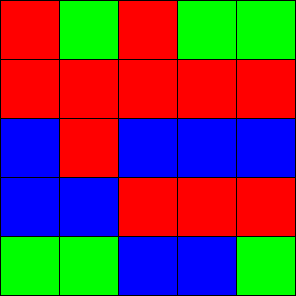
\includegraphics[width=\textwidth]{../figures/swap/swap_1.pdf}
            Original Image
        \end{column}
        \begin{column}{0.3\textwidth}
            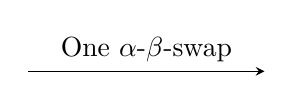
\begin{tikzpicture}
                \draw [->] (0,0) -- (3,0) node[midway, above] {One $\alpha$-$\beta$-swap};
            \end{tikzpicture}
        \end{column}
        \begin{column}{0.3\textwidth}
            \centering
            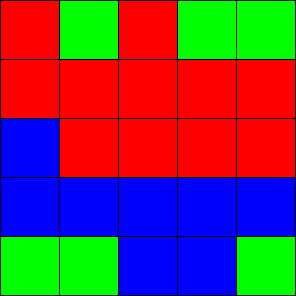
\includegraphics[width=\textwidth]{../figures/swap/swap_2.pdf}
            Optimized Image
        \end{column}
    \end{columns}
\end{frame}


\begin{frame}{$\textcolor{tumblue}{\alpha}$-expansion}
    \begin{itemize}
        \item$\alpha \hat=\text{red}$ 
        \item find optimum by expanding label $\alpha$ to other pixels \phantom{$f_p$} 
        \item[] \phantom{$\mathcal{P}_{\alpha,\beta}=\{p\in\mathcal{P} | f_p=\alpha \vee f_p=\beta \}$}
    \end{itemize}
    % \vspace{0.3cm}
    \begin{columns}
        \begin{column}{0.3\textwidth}
            \centering
            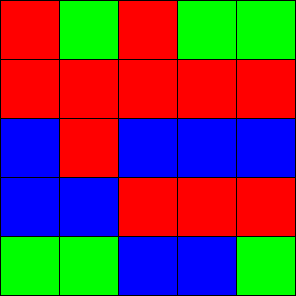
\includegraphics[width=\textwidth]{../figures/expansion/expansion_1.pdf}
            Original Image
        \end{column}
        \begin{column}{0.3\textwidth}
            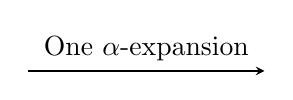
\begin{tikzpicture}
                \draw [->] (0,0) -- (3,0) node[midway, above] {One $\alpha$-expansion};
            \end{tikzpicture}
        \end{column}
        \begin{column}{0.3\textwidth}
            \centering
            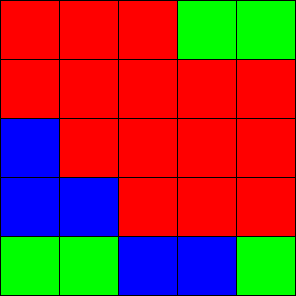
\includegraphics[width=\textwidth]{../figures/expansion/expansion_2.pdf}
            Optimized Image
        \end{column}
    \end{columns}

\end{frame}


\section{Swap Algorithm}
\secslide
\begin{frame}{Swap Algorithm}
    \begin{enumerate}
        \item[1.] Start with arbitrary labeling
        \item[2.] $\text{success} \coloneqq 0$
        \item[3.] for all $\{\alpha, \beta\} \subset \mathcal{L}$
        \begin{enumerate}
            \item[3.1] find $\hat f = \arg \min E(f')$ within one $\alpha$-$\beta$-swap
            \item[3.2] if $E(\hat f)<E(f)$ then $f=\hat f$
        \end{enumerate}
        \item[4.] if success $==1$ then goto \textcolor{tumblue}{2}
        \item[5.] return $f$
    \end{enumerate}
\end{frame}

\begin{frame}{Properties of Swap Algorithm}
    \begin{itemize}
        \item complexity is in one cycle $\mathcal{O}(|\mathcal{L}|^2)$
        \item termination is in $\mathcal{O}(|\mathcal{P}|)$ cycles
        \item most of the improvements occur in first cycle
        \item finds local minimum
        % \item but $E_\text{optimum}\leq E(f) \leq2k\cdot E_\text{optimum}$ and $k=\frac{\max V(\alpha,\beta)}{\min V(\alpha,\beta)}$
    \end{itemize}
\end{frame}

\section{Graph Cutting}
\secslide
\begin{frame}{Construction of Graph}
    \begin{columns}
        \begin{column}{0.6\textwidth}
        \only<1-6>{
             \scalebox{0.7}{
             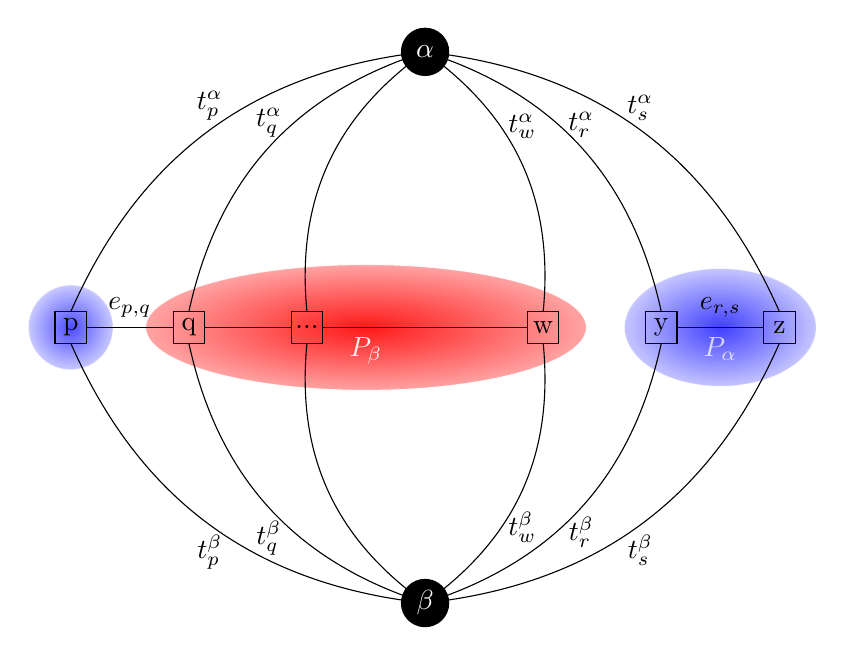
\begin{tikzpicture}

                 \def\radi{0.3}
                 \def\squ{0.2}
                 \def\d{1.5}
                 \def\a{3.5}
                 \def\b{-3.5}
                 
                 %ellipse large
             \visible<3->{    \draw[color=white, fill, opacity=0.9, inner color=red, outer color=red!40!] (-0.5*\d,0) ellipse (2.8cm and 0.8cm) node[below]{$P_\beta$};
                 
                 %ellipses small
                 \draw[color=white, fill, opacity=0.7, inner color=blue, outer color=blue!30!] (-3*\d,0) circle (1.8*\radi);
                 \draw[color=white, fill, opacity=0.75, inner color=blue, outer color=blue!30!] (2.5*\d,0) ellipse (1.22 and 0.75) node[below]{$P_\alpha$};
             }
             \visible<2->{
                 %pixel inner
                 \draw (-\d-\squ,0-\squ) rectangle node{...} (-\d+\squ,0+\squ);
                 \draw (\d-\squ,0-\squ) rectangle node{w} (\d+\squ,0+\squ);
                 
                 %pixel middle
                 \draw (-2*\d-\squ,0-\squ) rectangle node{q} (-2*\d+\squ,0+\squ);
                 \draw (2*\d-\squ,0-\squ) rectangle node{y} (2*\d+\squ,0+\squ);
                 
                 %pixel outer
                 \draw (-3*\d-\squ,0-\squ) rectangle node{p} (-3*\d+\squ,0+\squ);
                 \draw (3*\d-\squ,0-\squ) rectangle node{z} (3*\d+\squ,0+\squ);
             }
             \visible<4->{
                 %horizontal lines
                 \draw(-3*\d+\squ,0) -- node[above]{$e_{p,q}$} (-2*\d-\squ,0);
                 \draw(-2*\d+\squ,0) -- (-1*\d-\squ,0);
                 \draw(-1*\d+\squ,0) -- (1*\d-\squ,0);
                 % \draw(1*\d+\squ,0) -- (2*\d-\squ,0);
                 \draw(2*\d+\squ,0) -- node[above]{$e_{r,s}$} (3*\d-\squ,0);
             }
                 % %vertical lines top
             \visible<6->{
                 \draw(0,\a) to [bend right] node[above]{$t_p^\alpha$} (-3*\d,0+\squ);
                 \draw(0,\a) to [bend right] node[above]{$t_q^\alpha$} (-2*\d,0+\squ);
                 \draw(0,\a) to [bend right] (-1*\d,0+\squ);
                 \draw(0,\a) to [bend left] node[above=0.2cm]{$t_w^\alpha$} (1*\d,0+\squ);
                 \draw(0,\a) to [bend left] node[above]{$t_r^\alpha$} (2*\d,0+\squ);
                 \draw(0,\a) to [bend left] node[above]{$t_s^\alpha$} (3*\d,0+\squ);
                 
                 % %vertical lines bottom
                 \draw(0,\b) to [bend left] node[below]{$t_p^\beta$} (-3*\d,0-\squ);
                 \draw(0,\b) to [bend left] node[below=0.05cm]{$t_q^\beta$} (-2*\d,0-\squ);
                 \draw(0,\b) to [bend left] (-1*\d,0-\squ);
                 \draw(0,\b) to [bend right] node[below=0.15cm]{$t_w^\beta$} (1*\d,0-\squ);
                 \draw(0,\b) to [bend right] node[below]{$t_r^\beta$} (2*\d,0-\squ);
                 \draw(0,\b) to [bend right] node[below]{$t_s^\beta$} (3*\d,0-\squ);
             }
                 % %labels
             \visible<5->{
                 \draw[fill=black] (0,\a) circle (\radi) node{\textcolor{white}{$\alpha$}}; 
                 \draw[fill=black] (0,\b) circle (\radi) node{\textcolor{white}{$\beta$}}; 
             }
             \end{tikzpicture}%
             }%
        }
        \only<7>{
            \vspace{-0.5cm}
            \begin{figure}
                \centering
                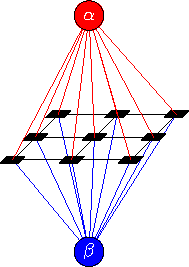
\includegraphics[width=.7\textwidth]{../figures/2d-graph/2d-graph.pdf}
            \end{figure}
        }
        \end{column}
        \begin{column}{0.4\textwidth}
            \begin{itemize}
                \item<2-> Introduce pixels
                \item<4-> Connect neighbours
                \item<5-> Introduce two terminal nodes
                \item<6-> Connect terminals and pixels
            \end{itemize}
        \end{column}
    \end{columns}
\end{frame}

\begin{frame}{Edge Weights}
    \begin{tabular}{l l l}
        \textbf{edge}       & \textbf{weight}       & \textbf{for}\\[0.2cm]
        \hline \\[0.2cm]
        $t_p^\alpha$ \phantom{blub}        & $D_p(\alpha) + \sum\limits_{\small \substack{q \in \mathcal{N}_p \\q \notin \mathcal{P}_{\alpha,\beta}}} V_{p,q}(\alpha,f_q)$ \phantom{blub} & $p \in \mathcal{P}_{\alpha,\beta}$ \\[0.9cm]
        $t_p^\beta$ \phantom{blub}        & $D_p(\beta) + \sum\limits_{\small \substack{q \in \mathcal{N}_p \\q \notin \mathcal{P}_{\alpha,\beta}}} V_{p,q}(\beta,f_q)$ \phantom{blub} & $p \in \mathcal{P}_{\alpha,\beta}$ \\[0.9cm]
        $e_{p,q}$    & $V_{p,q}(\alpha,\beta)$     & $\{p,q\} \in \mathcal{N} \wedge p,q \in \mathcal{P}_{\alpha,\beta}$
    \end{tabular}
\end{frame}


\begin{frame}{Possible Cuts}

    \begin{columns}
        \begin{column}{.5\textwidth}
            \setstretch{1.3}
            \begin{itemize}
                \item Find $\hat f = \arg \min E(f')$ within one $\alpha$-$\beta$-swap 
                \item[$\rightarrow$] do minimal graph cut
                \only<1>{
                \item[$\rightarrow$] $f_p = \beta$ and $f_q = \alpha$%
                }%
                % \only<2>{
                % \item[$\rightarrow$] $f_p = \alpha$ and $f_q = \beta$%
                % }%
                % \only<3>{
                % \item[\phantom{haha}] \phantom{lol}
                % }
                % \only<3->{
                % \visible<4>{
                % \item[$\rightarrow$] $f_p = \alpha$ and $f_q = \alpha$%
                % }}
            \end{itemize}
        \end{column}
        \begin{column}{.5\textwidth}
            \begin{figure}
                \centering
                % \only<3->{
                % 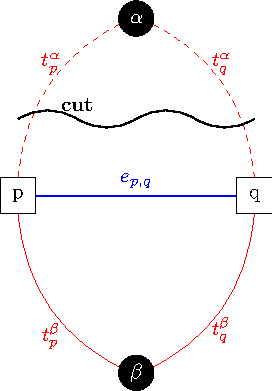
\includegraphics[width=.8\textwidth]{../figures/graph_cut/graph_3.pdf}%
                % }%
                % \only<2>{
                % 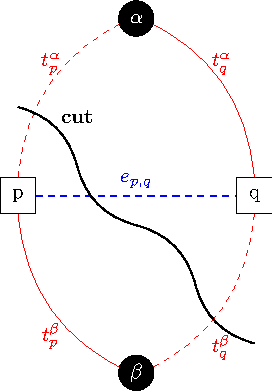
\includegraphics[width=.8\textwidth]{../figures/graph_cut/graph_2.pdf}%
                % }%
                \only<1>{
                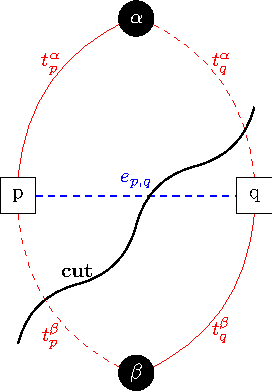
\includegraphics[width=.8\textwidth]{../figures/graph_cut/graph_1.pdf}%
                }
            \end{figure}
        \end{column}
    \end{columns}
\end{frame}

\begin{frame}{Minimum Cut}
    Cost of Minimut cut:
    \begin{equation}
       |\mathcal{C}| = \sum_{p \in \mathcal{P}_{\alpha,\beta}} \left| \mathcal{C} \cap \{t_p^\alpha,t_p^\beta \} \right|+ \sum\limits_{\small \substack{ \{p,q\} \in \mathcal{N}\\ \{p,q \} \subset \mathcal{P}_{\alpha,\beta}}} |\mathcal{C} \cap e_{p,q}|
    \end{equation}
    which can be rewritten to:
    \begin{equation}
        |\mathcal{C}| = E(f^\mathcal{C}) - K
    \end{equation}
    \vspace{-0.5cm}
    \begin{itemize}
        \footnotesize
        \item $f^\mathcal{C}$ labeling after cut
        \item $K$ is constant for all cuts $\mathcal{C}$ $\hat =$ independent of $\mathcal{C}$
    \end{itemize}
    \vspace{0.5cm}
    \textbf{$\implies$ Finding min $\mathcal{C}$ is equivalent to finding energy min}
\end{frame}

\begin{frame}{Finding Minimum Cut}
    \begin{itemize}
        \item famous Max-flow min-cut theorem
        % \item Content of TUM's \textit{Algorithmische Diskrete Mathematik} lecture
        \item Algorithms: \textit{Push-relabel}-based or \textit{Ford-Fulkerson}-based algorithms
        \item Kolmogorovs library \texttt{Maxflow}\footnote[frame]{\cite{kolmin} } is optimized for our graphs
        \item \texttt{PyMaxflow} is a python wrapper for \texttt{Maxflow} \footnote[frame]{\url{http://pmneila.github.io/PyMaxflow/}}
    \end{itemize}
\end{frame}


\begin{frame}[label=current]{Scaling of graph-cut with \texttt{PyMaxflow}}
    \texttt{PyMaxflow} scales more than quadratic $\implies$ confirms Boykov and Kolmogorov%\phantom{\cite{expcomp}}
    \begin{figure}
        \centering
        \begin{tikzpicture}
            \begin{axis}[
                width = 10cm, height = 6cm,
                xmin = 0, xmax = 1300, ymin = 0, ymax = 20,
                xlabel = {Image width in pixel}, ylabel = {time in seconds},
                % xtick = {0, 200, 400, 600,800,1000,1200},
                legend entries = {data, fit function $f=k \cdot x^{2.37}$},
                legend pos = {north west}
            ]
                \addplot[color=red, only marks, mark size = 0.7pt]
                    table [x expr ={\thisrowno{0}}, y index = 1] {../scaling/data4};
                \addplot[ color= green, domain=0:1300, line width = 1pt] {5.57856*10^(-7)*x^2.37054};
            \end{axis}
        \end{tikzpicture}
    \end{figure}
\end{frame}


\section{Implementation}
\secslide
\begin{frame}{Own Implementation}
    \begin{itemize}
        \item Implementation in Python available on \url{fcv.sumpi.org}
        \item uses \texttt{PyMaxflow}'s minimizing graph cut\footnote[frame]{\url{http://pmneila.github.io/PyMaxflow/}}
        \item objective: test different energy functions and images
        % \item execution by: python minimization.py test.png NUM\_CYCLES
    \end{itemize}

\end{frame}

\begin{frame}{Energy Function}
    In paper used
    \begin{equation}
        D_p(f_p) = (f_p - i_p)^2
    \end{equation}
    \begin{equation}
        V(f_p, f_q) = c\cdot |f_p-f_q| 
    \end{equation}
    but first is quadratic, second linear.\\
    \vspace{0.5cm}
    $\implies$
    another energy function which eliminates mismatch
    \begin{equation}
        \hat D_p(f_p) = \sqrt{|f_p^2 - i_p^2|}
    \end{equation}
    \footnotesize
    \begin{itemize}
        \item[] $f_p$ label of pixel $p$
        \item[] $i_p$ original intensity of pixel $p$
        \item[] $c$ some constant
    \end{itemize}
\end{frame}



\section{Experiments}
\secslide

\begin{frame}{Denoising Leopard using $\hat D_p(f_p)$ }
    Image with $500$x$489$ pixels in grayscale:
    
    \begin{columns}
        \begin{column}{0.4\textwidth}
            \begin{figure}[h]
                \centering
                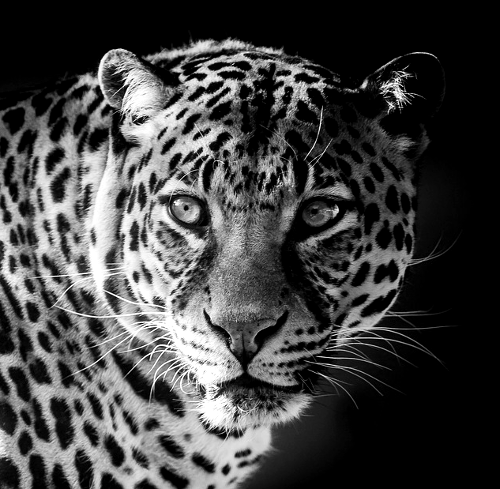
\includegraphics[width=.99\textwidth]{../testimages/leopard/leopard_500.png}
            \end{figure}
        \end{column}
        \begin{column}{0.2\textwidth}
            \centering
            \scalebox{0.4}{
            
\begin{tikzpicture}
                \fill[color=black!70!white] (1,0) --(3,0) --(3,1) --(4.5,-1) -- (3,-3) -- (3, -2) -- (1,-2);
            \end{tikzpicture}}
            $20$\% pixels are randomly changed 
        \end{column}
        \begin{column}{0.4\textwidth}
            \begin{figure}[h]
                \centering
                \includegraphics[width=.99\textwidth]{../testimages/leopard/leopard_500_20percent.png}
            \end{figure}
        \end{column}
    \end{columns}
\end{frame}


\begin{frame}{Denoising Leopard using $\hat D_p(f_p)$ }
    \begin{columns}
        \begin{column}{.5\textwidth}
            \only<2>{
                \begin{figure}
                    \centering
                    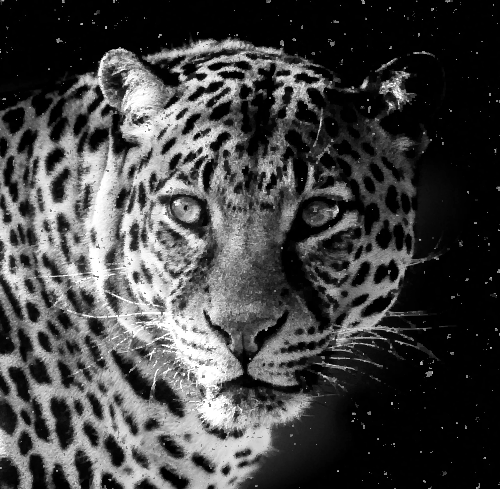
\includegraphics[width=1\textwidth]{../testimages/leopard/500_20percent/denoised_leopard_500_20percent_1_cycle.png}
                \end{figure}
            }
            \only<3>{
                \begin{figure}
                    \centering
                    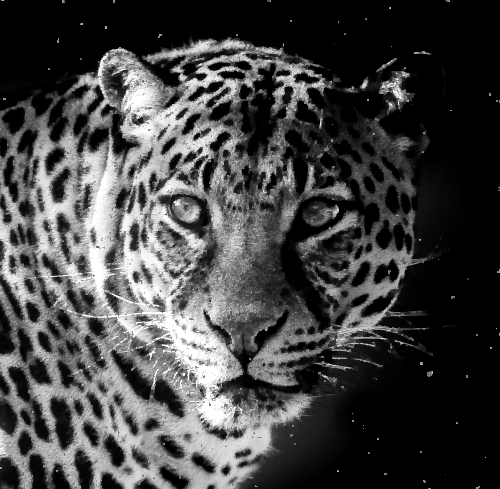
\includegraphics[width=1\textwidth]{../testimages/leopard/500_20percent/denoised_leopard_500_20percent_2_cycle.png}
                \end{figure}
            }
            \only<4>{
                \begin{figure}
                    \centering
                    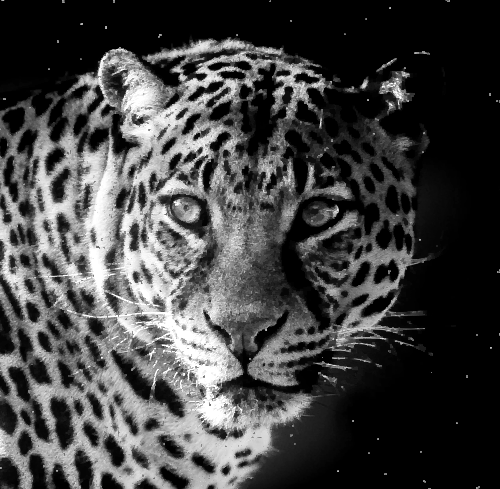
\includegraphics[width=1\textwidth]{../testimages/leopard/500_20percent/denoised_leopard_500_20percent_3_cycle.png}
                \end{figure}
            }
            \only<5>{
                \begin{figure}
                    \centering
                    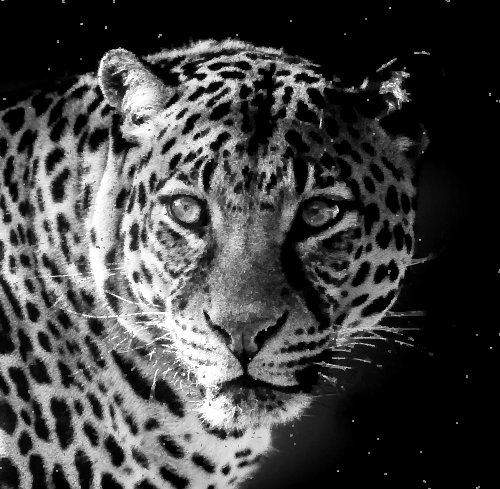
\includegraphics[width=1\textwidth]{../testimages/leopard/500_20percent/denoised_leopard_500_20percent_4_cycle.png}
                \end{figure}
            }
            \only<6>{
                \begin{figure}
                    \centering
                    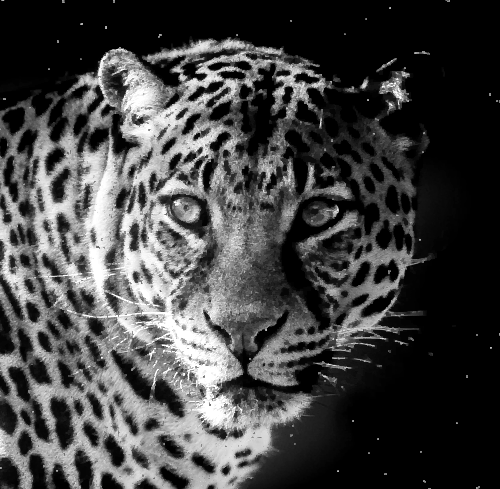
\includegraphics[width=1\textwidth]{../testimages/leopard/500_20percent/denoised_leopard_500_20percent_5_cycle.png}
                \end{figure}
            }
            \only<7>{
                \begin{figure}
                    \centering
                    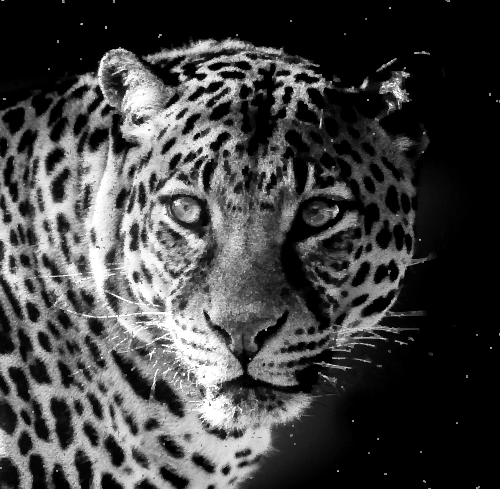
\includegraphics[width=1\textwidth]{../testimages/leopard/500_20percent/denoised_leopard_500_20percent_6_cycle.png}
                \end{figure}
            }
            \only<8>{
                \begin{figure}
                    \centering
                    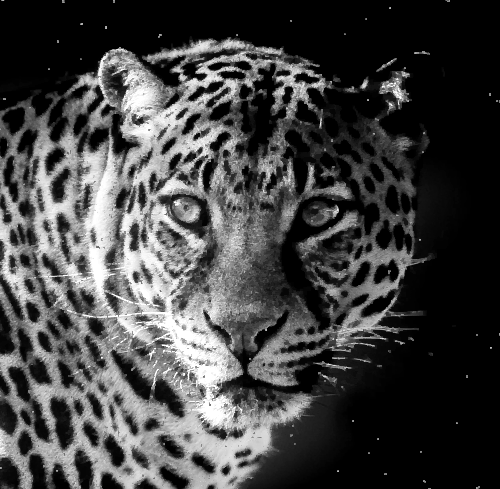
\includegraphics[width=1\textwidth]{../testimages/leopard/500_20percent/denoised_leopard_500_20percent_7_cycle.png}
                \end{figure}
            }
            \only<9>{
                \begin{figure}
                    \centering
                    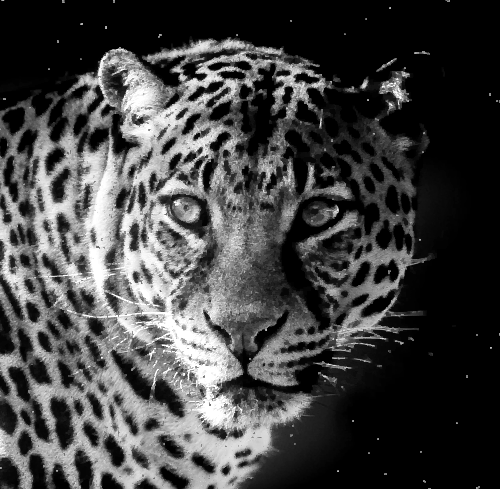
\includegraphics[width=1\textwidth]{../testimages/leopard/500_20percent/denoised_leopard_500_20percent_8_cycle.png}
                \end{figure}
            }
            \only<10>{
                \begin{figure}
                    \centering
                    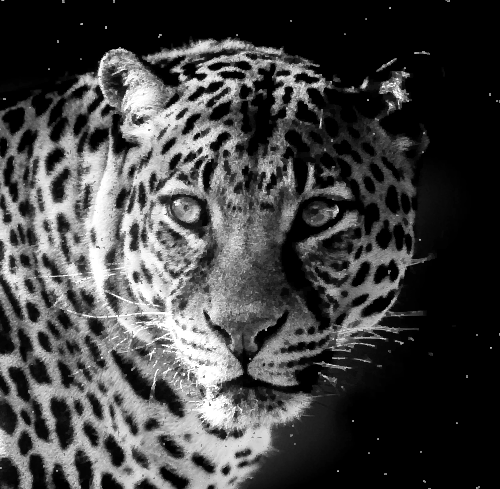
\includegraphics[width=1\textwidth]{../testimages/leopard/500_20percent/denoised_leopard_500_20percent_9_cycle.png}
                \end{figure}
            }
            \only<11->{
                \begin{figure}
                    \centering
                    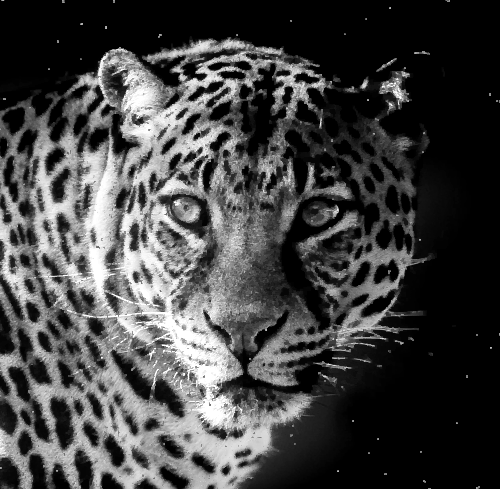
\includegraphics[width=1\textwidth]{../testimages/leopard/500_20percent/denoised_leopard_500_20percent_10_cycle.png}
                \end{figure}
            }
                \begin{center}
                    \only<2>{Denoised after 1 cycle}%
                    \only<3>{Denoised after 2 cycles}%
                    \only<4>{Denoised after 3 cycles}%
                    \only<5>{Denoised after 4 cycles}%
                    \only<6>{Denoised after 5 cycles}%
                    \only<7>{Denoised after 6 cycles}%
                    \only<8>{Denoised after 7 cycles}%
                    \only<9>{Denoised after 8 cycles}%
                    \only<10>{Denoised after 9 cycles}%
                    \only<11->{Denoised after 10 cycles}
                \end{center}
        \end{column}
        \begin{column}{.5\textwidth}
            \only<1-11>{
                \begin{figure}
                    \centering
                    \includegraphics[width=1\textwidth]{../testimages/leopard/500_20percent/leopard_500_20percent.png}
                \end{figure}
                \centering Noisy leopard
            }
            \only<12>{
                \begin{figure}
                    \centering
                    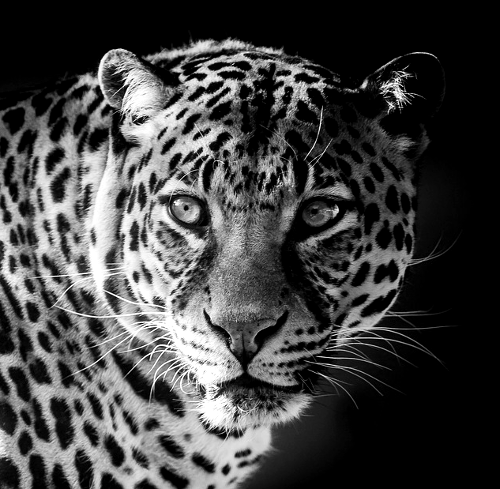
\includegraphics[width=1\textwidth]{../testimages/leopard/leopard_500.png}
                \end{figure}
                \centering Orginal leopard
            }
        \end{column}
    \end{columns}
\end{frame}


\begin{frame}{Denoising Lena $\hat D_p(f_p)$ }
    Lena in 500x500 pixels
    \begin{columns}
        \begin{column}{.45\textwidth}
                \begin{figure}
                    \centering
                    \includegraphics[width=.9\textwidth]{../testimages/Lena/500_10percent/denoised_Lenna_500_10percent_10_cycle.png}
                \end{figure}
                    {Denoised after 10 cycles}%
        \end{column}
        \begin{column}{.45\textwidth}
            \only<1>{
                \begin{figure}
                    \centering
                        \includegraphics[width=.9\textwidth]{../testimages/Lena/500_10percent/Lenna_500_10percent.png}
                \end{figure}
                \centering 10\% noisy Lenna
            }
            \only<2>{
                \begin{figure}
                    \centering
                    \includegraphics[width=.9\textwidth]{../testimages/Lena/500_10percent/Lenna_500.png}
                \end{figure}
                \centering Orginal Lenna 
            }
        \end{column}
    \end{columns}
\end{frame}



\begin{frame}{Energy over Cycles}
    \footnotesize
    Straight line is energy of original clear image
    \begin{figure}
        \begin{tikzpicture}
            \begin{axis}[
                width=10cm, height=6.8cm,
                xmin=-0.5, xmax=10.5, ymin=0, ymax=45000000,
                % y tick label style={/pgf/number format/fixed, /pgf/number format = \thinspace},
                scaled ticks=false,
                xtick = {0,1,2,3,4,5,6,7,8,9,10},
                y label style={at={(axis description cs:-0.05,.5)}},
                % ytick = {200000,400000, 600000, 800000},
                % yticklabels = {200000, 600000, 600000, 800000},
                xlabel = {Number of cycles}, ylabel = {Energy},
                minor y tick num = 3,
                legend entries = {House 20\% noise, Leopard 20\% noise}%, Leopard 5\% noise}
            ]
            \addplot[color=blue, only marks, mark size = 1.5pt]
                table[x index = 0, y index = 1] {../testimages/houses/houses_500_20/houses_500_20percent_energie};

            \addplot[color=red, only marks, mark size = 1.5pt]
                table[x index = 0, y index = 1] {../testimages/leopard/500_20percent/leopard_500_20percent_energie};

            % \addplot[color=red, only marks, mark size = 1.5pt, mark=square]
            %     table[x index = 0, y index = 1] {../testimages/leopard/500_5percent/leopard_500_5percent_energie};
            
            %leopard 500
            \addplot[color=blue!100!black, domain=-1:12, line width=0.6pt] {4891040.0};

            %house
            \addplot[color=red!100!black, domain=-1:12, line width=0.6pt] {12374628.0};

            % \addplot[color=blue!60!black, domain=-1:10, line width=1pt] {12374628.0};

            % \addplot[color=blue, only marks, mark size = 1.5pt, mark=square]
            %     table[x index = 0, y index = 1] {../testimages/Lena/500_5percent/Lenna_500_5percent_energy};
            % \addplot[color=blue, only marks, mark size = 1.5pt]
            %     table[x index = 0, y index = 1] {../testimages/Lena/500_10percent/Lenna_500_10percent_energy};
            % \addplot[color=blue!100!black, domain=-1:12, line width=0.6pt] {5445050.0};

            % \addplot[color=red, only marks, mark size = 1pt]
            %     table[x index = 0, y index = 1] {../testimages/dog2/2_output.txt};
            % \draw[color=green!40!black] (axis cs:-1,3551258) -- node[below]{Unnoised image} (axis cs:9,3551258);
            % \addplot[color=red, only marks, mark size = 1.5pt]
            %     table[x index = 0, y index = 1] {../testimages/leopard/250_10percent/250_10percent};
            % \addplot[color=red!60!black, domain=-1:10, line width=1pt] {3551258};
            
            % \addplot[color=green, only marks, mark size = 1.5pt]
            %     table[x index = 0, y index = 1] {../testimages/Lena/200_5percent/200_5percent.txt};
            % \addplot[color=green!60!black, domain=-1:10, line width=1pt] {1499586};
            \end{axis}
        \end{tikzpicture}
    \end{figure}
\end{frame}


\begin{frame}[label=current]{Conclusion}
    \begin{columns}
        \begin{column}{.5\textwidth}
            \phantom{lol}
            \vspace{0.0cm}
            \visible<2->{
                $E(f) = E_\text{smooth}(f) + E_\text{data}(f)$
            }
            \vspace{1.3cm}
            \visible<4->{
                \begin{figure}
                    \centering
                    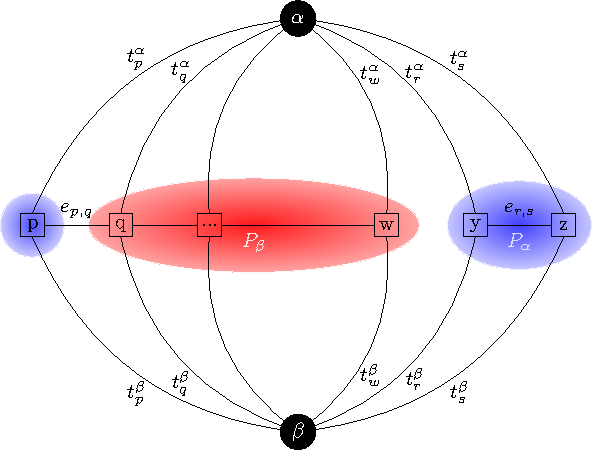
\includegraphics[width=.8\textwidth]{../figures/pixel/pixel_skizze.pdf}
                \end{figure}
            }
        \end{column}
        \begin{column}{.5\textwidth}
            \visible<3->{
            \vspace{-0.5cm}
                \begin{figure}
                    \centering
                    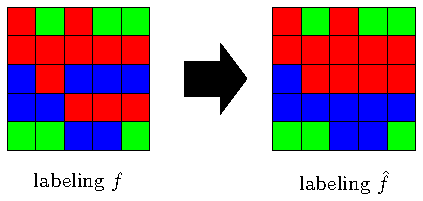
\includegraphics[width=\textwidth]{../figures/swap_change/swap_change.pdf}
                \end{figure}
            }
            \vspace{-0.5cm}
            \visible<5->{
                \begin{figure}
                    \centering
                    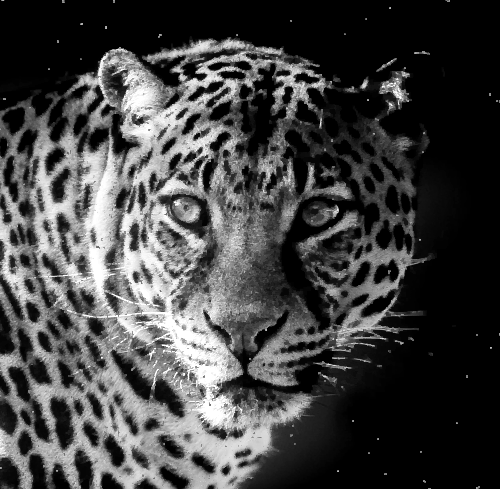
\includegraphics[width=.6\textwidth]{../testimages/leopard/500_20percent/denoised_leopard_500_20percent_10_cycle.png}
                \end{figure}
            }
        \end{column}
    \end{columns}

\end{frame}



% \begin{frame}{Conclusion}
%     \begin{itemize}
        % \item possible to find near-optimum solution
        % \item paper has over 7000 citations $\implies$ starting point of graph cuts 
        % \item can be applied to image segmentation and other energy minimizing problems
        % \item $\alpha$-expansion is today preferred 
    % \end{itemize}
% \end{frame}


\begin{frame}[shrink=30]{Bibliography}
    \nocite{*}
    \printbibliography
\end{frame}


%%%%%%%%%%%%%%%%%%%%%%%
%%%  APPENDIX BEGIN %%%
%%%%%%%%%%%%%%%%%%%%%%%
\appendixStart

% \begin{frame}
%     \begin{figure}[h]
%         \centering
%         \includegraphics[width=.5\textwidth]{../figures/graph_example.png}
%     \end{figure}

%     \begin{figure}[h]
%         \cite{xdot}
%         \centering
%         \includegraphics[width=.5\textwidth]{../figures/graph_example_complex.png}
%     \end{figure}
% \end{frame}


\begin{frame}{More examples}
    \begin{columns}
        \begin{column}{.3\textwidth}
            \begin{figure}
                \centering
                
\includegraphics[width=\textwidth]{../testimages/shapes/shapes_500_15percent/denoised_shapes_500_15percent_10_cycle.png}
            \end{figure}
                \centering
                Denoised after 10 cycles using $\hat D_p(f_p)$ \phantom{hahahahha$V(f_q,f_p) ll lsadasdsad asd sa d$} \phantom{hahahhahahahahhahahahaha sadasdasdasasdaasasdasdasdasdsadsdh $V_p$} 

        \end{column}
        \begin{column}{.3\textwidth}
            \begin{figure}
                \centering
                \only<4>{
\includegraphics[width=\textwidth]{../testimages/shapes/shapes_500_15_min_500_euclidean/min_500_euclidean_bad_denoised_shapes_500_15percent_10_cycle.png}}%
                \only<3>{
\includegraphics[width=\textwidth]{../testimages/shapes/shapes_500_15_v80/v_80_bad_denoised_shapes_500_15percent_10_cycle.png}}%
                \only<2>{
\includegraphics[width=\textwidth]{../testimages/shapes/v45_shapes_500_15percent/v45_bad_denoised_shapes_500_15percent_10_cycle.png}}%
                \only<1>{
\includegraphics[width=\textwidth]{../testimages/shapes/euclidean_shapes_500_15percent/euclidean_bad_denoised_shapes_500_15percent_10_cycle.png}}
            \end{figure}
                \centering
                \only<4>{Denoised after 10 cycles using $D_p(f_p)$ and min 500 euclidean distance for  $V(f_p,f_q)$}%
                \only<3>{Denoised after 10 cycles using $D_p(f_p)$ and $c=80$ in $V(f_p,f_q)$}%
                \only<2>{Denoised after 10 cycles using $D_p(f_p)$ and $c=45$ in $V(f_p,f_q)$}%
                \only<1>{Denoised after 10 cycles using $D_p(f_p)$ and euclidean distance for $V$\phantom{$V_p$}}%
        \end{column}
        \begin{column}{.3\textwidth}
            \begin{figure}
                \centering
                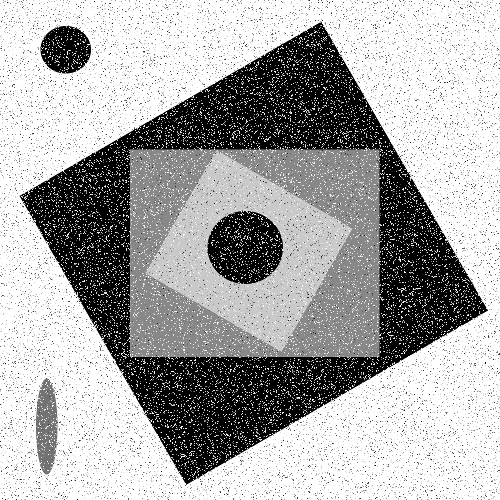
\includegraphics[width=\textwidth]{../testimages/shapes/shapes_500_15percent.png}
            \end{figure}
                \centering
                15\% noised shapes \phantom{hahahhahahahahhahahahaha sadasdasdasasda asasdasdasdasdsadsdh} \phantom{hihasdsadsad} \phantom{hahahahha$V(f_q,f_p)$}
        \end{column}
    \end{columns}
\end{frame}

\begin{frame}{Example House}
 \begin{columns}
        \begin{column}{.3\textwidth}
            \begin{figure}
                \centering
                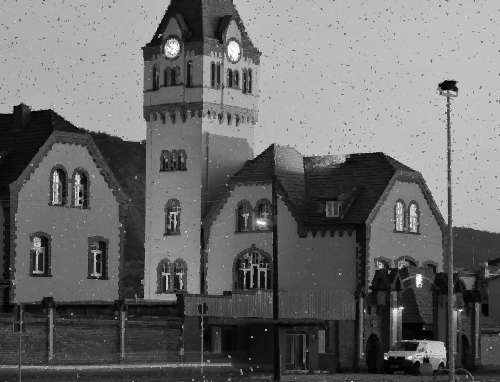
\includegraphics[width=\textwidth]{../testimages/houses/houses_500_20/denoised_house_500_20percent_10_cycle.png}
            \end{figure}
                \centering
                Denoised after 10 cycles using $\hat D_p(f_p)$ 
        \end{column}
        \begin{column}{.3\textwidth}
            \begin{figure}
                \centering
                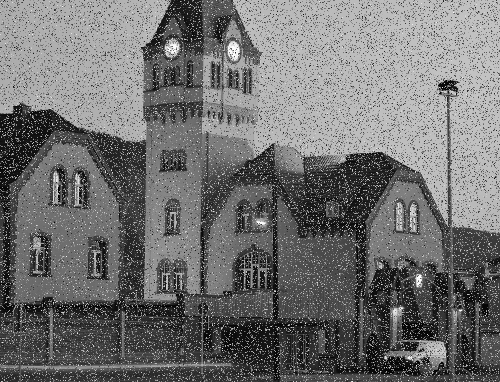
\includegraphics[width=\textwidth]{../testimages/houses/houses_500_20/house_500_20percent.png}
            \end{figure}
                \centering
                20\% noised house \phantom{cycles using $\hat D_p(f_p)$} 
        \end{column}
        \begin{column}{.3\textwidth}
            \begin{figure}
                \centering
                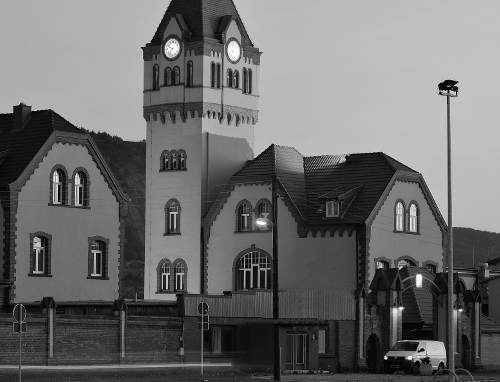
\includegraphics[width=\textwidth]{../testimages/houses/houses_500_20/house_500.png}
            \end{figure}
                \centering
            Original house \phantom{cycles using $\hat D_p(f_p)$} 
        \end{column}
    \end{columns}
\end{frame}

\begin{frame}{Comparison House}
 \begin{columns}
        \begin{column}{.3\textwidth}
            \begin{figure}
                \centering
                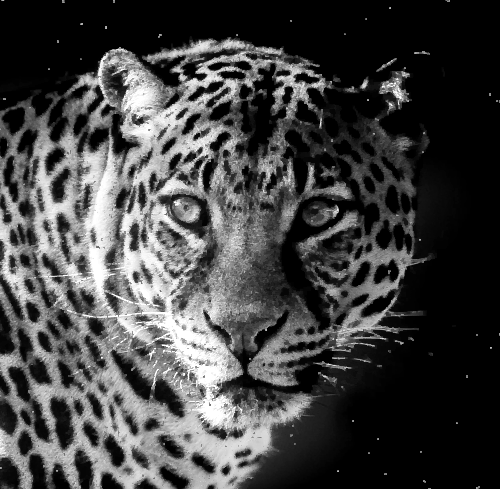
\includegraphics[width=\textwidth]{../testimages/leopard/500_20percent/denoised_leopard_500_20percent_10_cycle.png}
            \end{figure}
                \centering
                Denoised after 10 cycles using $\hat D_p(f_p)$ 
        \end{column}
        \begin{column}{.3\textwidth}
            \begin{figure}
                \centering
                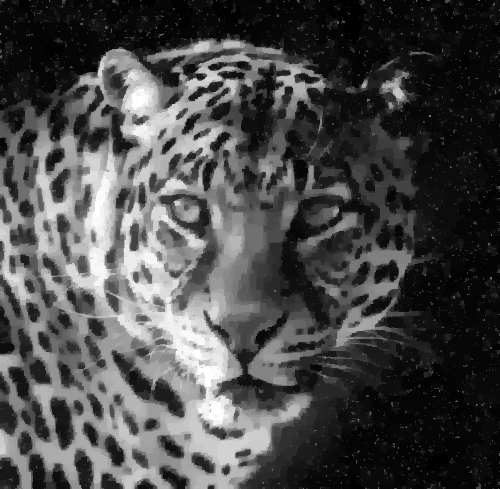
\includegraphics[width=\textwidth]{../testimages/leopard/v80_500_20/v80_bad_denoised_leopard_500_20percent_10_cycle.png}
            \end{figure}
                Denoised after 10 cycles using $\hat D_p(f_p)$ and $V=80\cdot|f_p-f_q|$  
        \end{column}
        \begin{column}{.3\textwidth}
            \begin{figure}
                \centering
                \includegraphics[width=\textwidth]{../testimages/leopard/v80_500_20/leopard_500_20percent.png}
            \end{figure}
                Original image
        \end{column}
    \end{columns}
\end{frame}




\appendixEnd
\end{document}
